

\section{The Programmable SumCheck Accelerator}

\subsection{Challenges}

At its core, SumCheck offers several degrees of parallelism. 
Different MLE tables can compute their extensions in parallel, extensions for different MLE pairs \textit{within} a table can be computed in parallel, and the products \textit{across} different extensions can be computed in parallel. Given a SumCheck polynomial, an optimal circuit can be constructed to maximize reuse and throughput, as done in zkSpeed \cite{zkspeed2025}.

In contrast, a generalizable SumCheck unit must support a diverse set of composite polynomial structures used to express different types of constraints or implement different kinds of operations. 
The unit must support an arbitrary number of terms and an arbitrary degree. This means that the optimal resource allocation (e.g., number of modular multipliers) for one composite polynomial may be suboptimal or wasteful for another one. Additionally, many composite polynomials have individual polynomials that repeat. For example, in $f = a\cdot b \cdot e + c \cdot e + e \cdot g $, the $e$ polynomial appears three times.
While we could parallelize all computations for the first term ($a \cdot b \cdot e$) before proceeding to the next term, this would leave out a clear opportunity for data reuse. Indeed, zkSpeed's design captures immediate reuse, but is tailored to HyperPlonk's Vanilla gate polynomials. zkSpeed overprovisions resources for simple polynomials, and cannot support complex composite polynomials.

\begin{figure}[t!]
\centerline{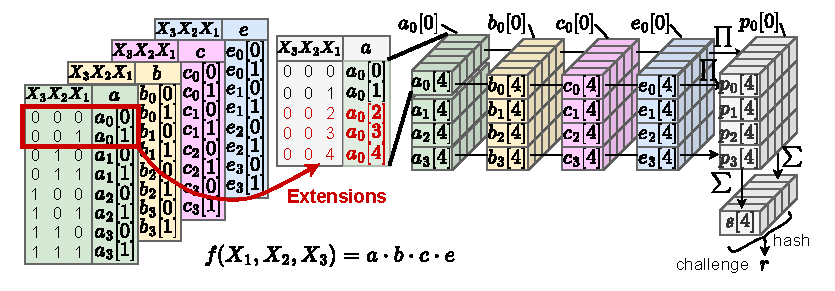
\includegraphics[width=1.02\columnwidth]{sumcheck_dataflow_new.pdf}}
\caption{The SumCheck dataflow of size-$2^{3}$ polynomial $f(X)=abce$.
For a degree-4 polynomial $f$, every MLE evaluation pair is extended to five evaluations.
Extended evaluations are multiplied, summed, and hashed to get a challenge that is used to update MLE tables for the next SumCheck round. }
\label{fig:SumCheck_dataflow_example}
\end{figure}

\subsection{Datapath}
Our programmable SumCheck unit seeks to balance the trade-off between resource allocation and capturing immediate data reuse.
\autoref{fig:new_sumcheck}
shows the datapath 
for our programmable SumCheck unit. 
It consists of several processing elements (PEs), with MLE Update units, Extension Engines (EEs) and Product Lanes (PLs).
Instead of streaming all individual polynomials' MLE entries simultaneously, we proceed one term at a time, fetching a \textit{tile} of data from each MLE table and storing in local scratchpad buffers.
We allocate 16 scratchpad buffers, more than sufficient to accommodate polynomial structures we see in current ZKP systems.
The scratchpad buffers are banked to match the number of PEs for parallel accesses.
This ensures that individual polynomials reused in subsequent terms need not be fetched from off-chip memory for a given tile.

For a given term, the polynomials are read into the Update units and EEs, where their extensions are generated by a series of modular adders and subtractors.
Specifically, in round 1 of SumCheck, each PE reads two values at a time from MLE tables and directly feeds them to the EEs to generate extensions.
In all subsequent rounds, four values are read per MLE, because we pipeline the MLE updates directly into the extension computation.
Updating with four inputs ensures that two values are generated and fed to the EEs to match the 
same
throughput of round 1.
These updated values are also written to FIFOs that buffer writebacks to off-chip, forming the (halved) tables for the next SumCheck round.
In later rounds of SumCheck where MLE tables can fit fully on-chip, writebacks to off-chip are eliminated and updated values are directly routed to the scratchpad banks.

After each MLE's extensions are generated, they are packed into their respective groups, e.g., the extensions for all MLEs at $X_i = 2$ are routed together.
Each group of extensions is then fed into a Product Lane (PL).
Each PL is equipped with $E - 1$ fully pipelined modular multipliers, where $E$ is the number of EEs.
Each PL's output is accumulated into a register corresponding to the extension, e.g., all products at $X_i = 2$ are routed to register $2$.
We allocate 32 registers (up to degree 31); higher degrees are supported by storing in scratchpads.

\subsection{Mapping Polynomials to EEs}
We devise a scheduler that determines which MLE tables are fed to EEs and PLs using a graph-based decomposition (see \autoref{fig:scheduler}). 
In this example, we assume there are 3 EEs, so only 3 MLEs can be handled by a SumCheck PE at a time. 
The polynomial is adding a degree-6 term and a degree-3 term.
Since there are more MLEs than EEs, we must store the intermediate products for \textit{all} extensions, not just the initial extensions at $X_i = 0, 1$ that are provided from the original MLE tables. This is done using a dedicated \textit{Tmp} MLE buffer.

A natural way to schedule the MLEs is using the balanced tree-based approach on the left in \autoref{fig:scheduler}.
However, this would require storing two distinct intermediate products that would need to be combined.
As the polynomial degree grows, this tree-based approach would require more and more intermediate buffers.
Instead, we can use the accumulation-based schedule on the right.
This scheme only requires 1 Tmp MLE buffer that accumulates extension products within the same term.
Notice that this scheme uses the same number of steps as the balanced tree while minimizing temporary storage.

\begin{figure}[t!]
\centerline{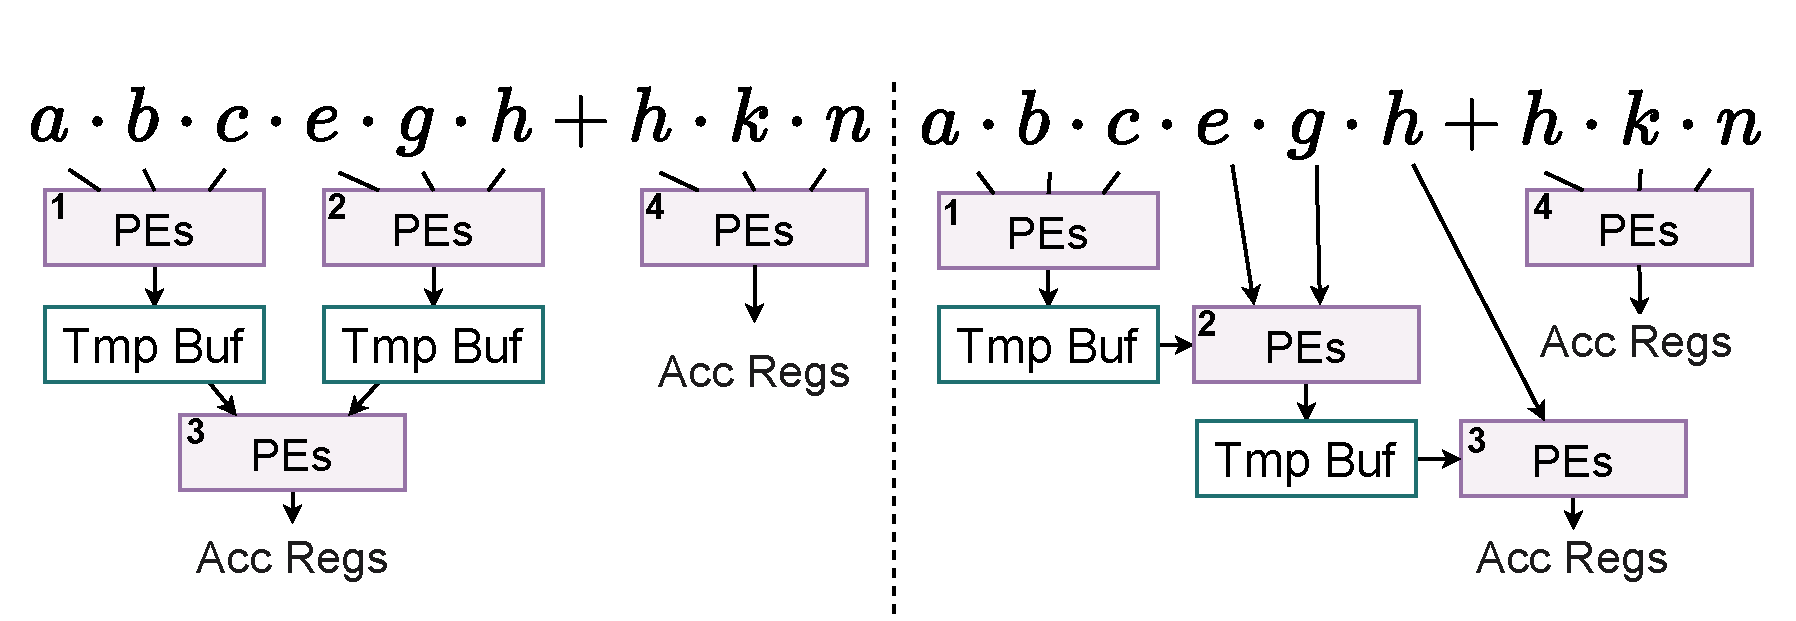
\includegraphics[width=0.98\columnwidth]{hpca_polynomial-Page-3.drawio.pdf}}
\caption{Graph decomposition used to schedule computation on our SumCheck unit. The method on the right minimizes the number of temporary MLE buffers. Numbers inside each node indicate the step in the schedule. When processing term $hkn$, $h$ is already prefetched during the prior step.}
\label{fig:scheduler}
\end{figure}


This way, the scheduler traverses the polynomial term-by-term, deciding which MLEs are handled by the PEs in each step.
In each step $j$, the PEs read the MLEs assigned to step $j$, while
a tile of data for each MLE needed in step $j + 1$ is prefetched if it is not already brought on-chip.
For example, the $h$ MLE is prefetched during step $2$ 
(on the right), 
while only the $k$ and $n$ MLEs are prefetched during step $3$.
For higher-degree polynomials, this scheme balances prefetch bandwidth across steps rather than front-loading it in the initial steps, as would occur with a binary-tree schedule.

\begin{figure*}[t!]
    \centering
    % First figure in the left column
    \begin{minipage}{0.69\textwidth}
        \centering
        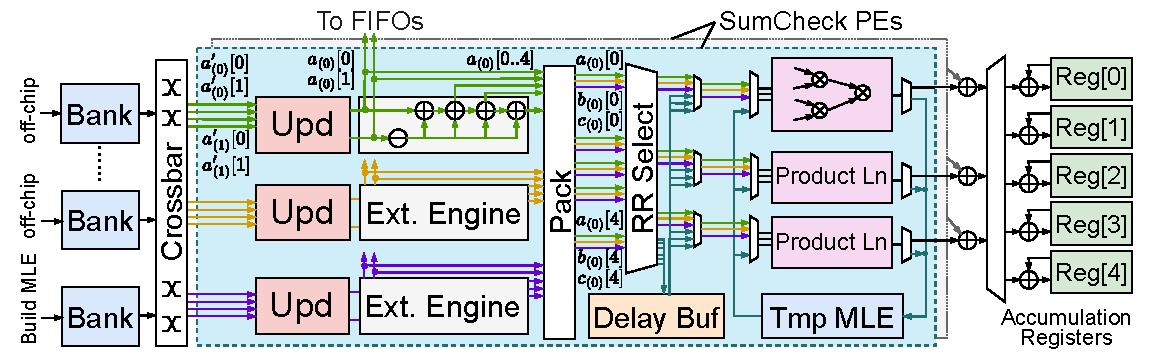
\includegraphics[width=\textwidth]{sumcheck_uarch.pdf}
        \caption{Programmable SumCheck Architecture.
        The Update unit updates the MLE $a^{\prime}$ to halved-size MLE $a$ for the next SumCheck round.
        For deg-4 term $abce$, Extension Engines generate five evaluations $0$-$4$.}
        \label{fig:new_sumcheck}
    \end{minipage}
    \hfill
    % Second figure in the right column
    \begin{minipage}{0.3\textwidth}
        \centering
        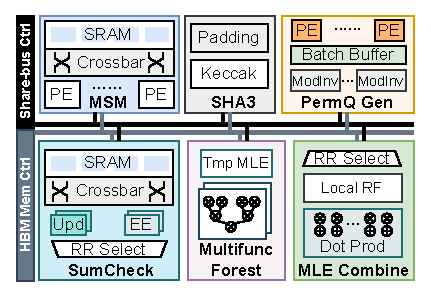
\includegraphics[width=\textwidth]{toplevel.pdf}
        \caption{Overall Architecture of zkPHIRE.}
        \label{fig:overall_arch}
    \end{minipage}
\end{figure*}


\subsection{Mapping Extensions to PLs}
Our SumCheck unit must handle any number of extensions, and we may run into scenarios where there are $K$ extensions but only $P < K$ lanes. In this case, we have an initiation interval $II = K/P$ and use delay buffers to queue extra extensions. 
In \autoref{fig:new_sumcheck}, with $K=5$ and $P=3$, the first cycle maps extensions $0$–$2$ to PLs, while extensions $3$–$4$ are buffered for the next cycle.
Scheduling proceeds in a pipelined fashion, with buffered and incoming extensions interleaved across PLs.


\subsection{Programming the SumCheck unit}
The SumCheck unit is programmed via an automated scheduler given the target polynomial and hardware configuration.
Using the approach shown in Figure~2, the scheduler generates a list of computational steps, including MLE-to-EE mappings, prefetch ordering, and schedules for specific $(K, P)$ settings. 
These steps are annotated with signals for control registers (e.g., MLE bank selection, arbitration, bypassing update), address offsets, and FSM configuration. 
They are then loaded into on-chip controllers as instructions to guide SumCheck execution.


\subsection{Built-in support for ZeroChecks}
Many ZKP protocols use SumCheck to verify circuit correctness by checking that a polynomial $f(X)$ evaluates to zero across all inputs. However, simply verifying $\sum_X f(X) = 0$ is insufficient. Individual gates could evaluate to nonzero values (meaning they were incorrectly executed), but cancel each other out, so the total sum would still be zero. To prevent this, protocols like \cite{spartan, orion, strawman} use \textit{ZeroCheck}, which multiplies $f(X)$ with a randomized auxiliary polynomial $f_r(X)$
\footnote{In the ZKP literature \cite{spartan, hyperplonk, jolt}, $f_r(x)$ is written as $eq(x, r)$}
and checks that $\sum_X (f(X) \cdot f_r(X)) = 0$.
$f_r(X)$ is constructed on-the-fly from a vector of random challenges generated by a SHA module.
The construction of an $f_r(X)$ polynomial is referred to as the \textit{Build MLE} kernel in zkSpeed, and we integrate this auxiliary polynomial construction directly into the SumCheck datapath. During the first SumCheck round, one product lane is dedicated to computing $f_r(X)$. Its outputs are routed to a dedicated scratchpad bank and one EE, while the remaining EEs fetch MLE elements from the other scratchpad banks.
One less lane is available for product computations for the first SumCheck round, but this avoids separate $O(N)$ precomputation of $f_r$ and the memory overhead of writing and reading back values.
Subsequent SumCheck rounds treat $f_r$ as any other MLE fetched from and updated to off-chip.


\section{zkPHIRE Architecture}
We include the programmable SumCheck unit as part of zkPHIRE, a larger accelerator framework for the HyperPlonk protocol. \autoref{fig:overall_arch} shows the overall architecture.


\subsection{HyperPlonk Protocol Overview}
HyperPlonk has a very complex dataflow as outlined in~\cite{zkspeed2025}. Here, we describe the high-level protocol and which hardware modules each step requires. The 5 main steps are Witness Commitments, Gate Identity Check, Wire Identity Check, Batch Evaluations, and Polynomial Opening. 

In \textbf{Witness Commitments}, the prover commits to their private input values (witnesses) using multi-scalar multiplications (MSMs) so that they cannot claim other witness values later. We run this step with the MSM unit.
In \textbf{Gate Identity Checks}, the prover shows that all gates in the circuit were computed correctly via ZeroChecks. We run this step with our SumCheck unit and a Multifunction Forest unit.
In \textbf{Wire Identity Checks}, the prover proves that the wiring between gates is consistent with the circuit's intended connections
by enforcing a permutation argument over the wire values. This is done by constructing wiring permutation polynomials and forming a quotient and \textit{grand product} 
argument
that encodes the permutation constraint. These polynomials are committed to, and then correctness of the grand product is verified via a PermutationCheck (PermCheck).
We run this step with a Permutation Quotient Generator unit,
the SumCheck and Multifunction Forest units, and the MSM unit.

In \textbf{Batch Evaluations}, the prover evaluates all committed polynomials at various points provided by the verifier. We run this step with the Multifunction Forest unit.
In the \textbf{Polynomial Opening}, the prover reveals the values of multiple committed polynomials at specific points and proves that it is consistent with the original commitment. The prover then runs a SumCheck to combine these polynomial evaluation claims into one (we call this \textit{OpenCheck} as per zkSpeed).
The combined polynomial commitment is then opened using the MSM unit.
Overall this step uses an MLE Combine unit, the SumCheck and Multifunction Forest units, and the MSM unit.

\textbf{Masking ZeroCheck:} In zkSpeed and the HyperPlonk baseline, Gate Identity and Wire Identity steps run serially, despite verifying independent circuit properties. zkPHIRE includes support to overlap the Gate Identity’s ZeroCheck with the MSMs during Wiring Identity. MSMs dominate runtime and have low bandwidth pressure due to high data reuse~\cite{szkp, zkspeed2025}, so this scheduling effectively masks ZeroCheck latency.

\subsection{Accelerator Units}
\subsubsection{\textbf{SumCheck Unit with Sparsity Handling}} ZKP protocols often exhibit significant sparsity: enable MLEs ($q_i$) are mostly binary, while constant and witness MLEs ($q_c$, $w_i$) are typically 90\% sparse~\cite{szkp, pipezk, zkspeed2025}. zkPHIRE extends the SumCheck unit to exploit this sparsity for improved efficiency.


zkSpeed opts to use large on-chip scratchpads to store these MLEs, because they are reused throughout steps of the HyperPlonk protocol.
However, as the problem size scales, the area consumed by the scratchpad grows, with 10s of MBs dedicated to address translation buffers alone, and a total on-chip storage of nearly 300 MB.
Furthermore, the MLEs are only useful for round 1 of SumChecks. For subsequent rounds, the MLEs are updated and written to off-chip memory, so the global scratchpad is idle for roughly 50\% of the SumCheck runtime.
zkPHIRE opts to use smaller scratchpad buffers to store tiles of each MLE.
While this results in more access to off-chip memory and incurs more fill/drain latency penalties, it allows for more area to be dedicated to core computational structures. The improved speedups offset the latency hits incurred by using smaller scratchpads. 

zkSpeed's scratchpads compress MLEs but require address translation units to decode when MLE entries are sparse or dense. zkPHIRE eliminates the address translation overhead by fetching \textit{per-tile offset buffers} for witness MLEs.
For a tile of data fetched from off-chip, the SumCheck controller uses the offset buffer to determine where 255-bit elements begin in the bitstream; all other bits are interpreted as $0/1$ MLE entries and written into the corresponding addresses in the scratchpads.
The enable MLEs are stored as-is without using address translation. 
These optimizations incur minimal bandwidth costs while enabling more compact storage.



\subsubsection{\textbf{Multifunction Forest}}
In HyperPlonk, several sub-steps naturally map to binary-tree computations, such as MLE evaluation, computing the product MLE ($\pi$), and building MLEs~\cite{mo2025mtu}. 
We adopt the same base tree architecture as zkSpeed's MTU~\cite{mo2025mtu, zkspeed2025}, but differ in how it is integrated.
Whereas zkSpeed uses a single tree unit alongside a dedicated SumCheck module, zkPHIRE instantiates multiple tree units as a Multifunction Forest.
These units are reused to implement product-lane computations, removing the need for the extra modular multipliers in zkSpeed’s SumCheck module while keeping the pipeline fully utilized.
This shared design allows the same multipliers to serve both SumCheck products and other tree-based operations, improving utilization and reducing area.
As a result, zkPHIRE achieves the same latency as zkSpeed for the same workload with 15\% fewer multipliers.


\subsubsection{\textbf{MSM}}
We use the same MSM architecture as zkSpeed, since we target the same protocol, HyperPlonk. In HyperPlonk, the number of MSMs only depends on the number of witnesses. The underlying hardware is unchanged, we just compute more MSMs using it. Jellyfish gates have 5 witnesses, so we run 5 Sparse MSMs and 3 Dense MSMs.

\subsubsection{\textbf{MLE Combine}}
The MLE Combine module, shown in \autoref{fig:overall_arch}, is used for various element-wise operations and dot products before and after the OpenCheck in Polynomial Opening. For these steps, we fetch MLE tables from off-chip into up to 6 local SRAM buffers and perform the operations between MLE entries and/or challenges from prior protocol steps stored in registers. All operations are fully pipelined.

\subsubsection{\textbf{Permutation Quotient Generator}}

\begin{figure}[t!]
    \centering
    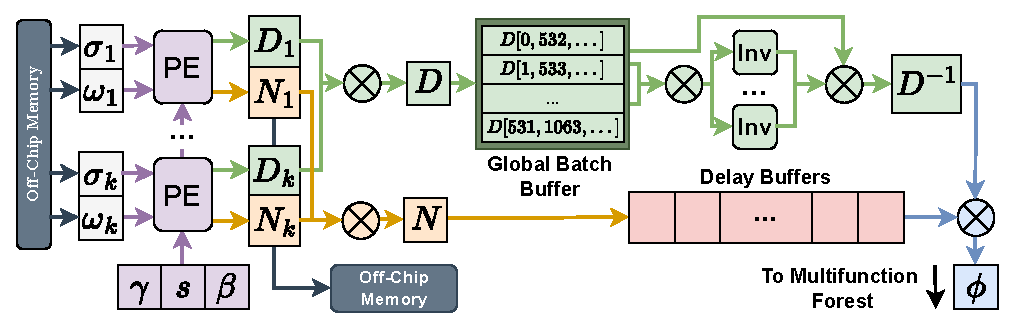
\includegraphics[width=\columnwidth]{permquotgen.pdf}
    \caption{The Permutation Quotient Generator Module.}
    \label{fig:genND_fracMLE}
\end{figure}
PermCheck requires constructing Numerator ($N$), Denominator ($D$), Fraction ($\phi$), and Product ($\pi$) MLEs \cite{zkspeed2025}. Since $\phi$ is computed on-the-fly from N and D, we design a pipelined unit that generates all three simultaneously, producing one element per cycle after warmup (\autoref{fig:genND_fracMLE}). The Multifunction Forest is used to construct $\pi$ from $\phi$, as in zkSpeed. To accommodate both Vanilla and custom gates, we allocate 5 PEs (one per witness), with the ability to support more than 5 through overlapped scheduling and cyclic reuse of PEs. Intermediate $N_{1\dots k}$ and $D_{1\dots k}$ MLEs are written to HBM and combined with modular multiplications to produce the final $N$ and $D$ MLEs, followed by modular inversion of $D$.

We build on zkSpeed’s Montgomery batching approach~\cite{Montgomery_1987}, which uses a batch size of 64 and dedicated multipliers to mask inversion latency at high area cost. To improve efficiency, we reduce the batch size to 2 and eliminate per-inverse multipliers, instead using two shared multipliers, one for batching and one for output isolation. Since zkSpeed's modular multipliers are 17.7$\times$ larger than their inverse units (0.478 mm$^2$ vs. 0.027 mm$^2$ in TSMC 22nm), we increase the number of inverse units and schedule them in a round-robin fashion to initiate one inversion every two cycles without backpressure. We find that 266 inverse units is sufficient for this. A shared batch buffer stores inputs; once an inverse completes, it is multiplied by its paired batch element and the slot is reused. Our design achieves a 4.2$\times$ area reduction over zkSpeed without sacrificing throughput.

